\documentclass[final,3p,authoryear]{elsarticle}

\usepackage{lipsum}
 \usepackage{graphics}
\usepackage[]{algorithm2e}
 \usepackage{setspace}
%% or use the graphicx package for more complicated commands
 \usepackage{graphicx}
%% or use the epsfig package if you prefer to use the old commands
 \usepackage{epsfig}
 \usepackage{subfigure}

%% The amssymb package provides various useful mathematical symbols
\usepackage{amssymb}
%% The amsthm package provides extended theorem environments
 \usepackage{amsthm,amsmath}
 \usepackage{multirow}
 \usepackage{setspace}
 \usepackage{CJK}
 \usepackage{float}
 \usepackage{pdfpages}
 \usepackage{mathtools}
% \usepackage{natbib}
 \restylefloat{table}
 \onehalfspacing



\makeatletter
\def\ps@pprintTitle{%
	\let\@oddhead\@empty
	\let\@evenhead\@empty
	\def\@oddfoot{}%
	\let\@evenfoot\@oddfoot}
\makeatother

\usepackage{etoolbox}
\patchcmd{\abstract}{Abstract}{}{}{}

\begin{document}

\begin{frontmatter}

\title{MATH 6740: Financial Mathematics and Simulation\\
	Homework 5 solutions/presentation}

\author[rvt]{Jubiao ``Jack'' Yang}

\address[rvt]{Rensselaer Polytechnic Institute, Troy, NY 12180}

\begin{abstract}
	Solve Exercise Problem 4.9 in \cite[Chapter 4]{shreve2004stochastic}.
\end{abstract}


\end{frontmatter}


\section{Exercise 4.9 (Analytical solution to Black-Scholes equation)}
	\subsection{(i)}
		\begin{proof}
			\begin{align}
				\text{LHS}\equiv K e^{-r\left(T-t\right)} N'(d_-) &= K e^{-r\left(T-t\right)} \frac{1}{\sqrt{2\pi}} e^{-\frac{d_-^2}{2}}
				\nonumber\\
				&= K e^{-r\left(T-t\right)} \frac{1}{\sqrt{2\pi}} e^{-\frac{\left(d_+ - \sigma \sqrt{T-t}\right)^2}{2}}
				\nonumber\\
				&= K e^{-r\left(T-t\right)} \frac{1}{\sqrt{2\pi}} e^{-\frac{d_+^2}{2}} e^{-\frac{\sigma^2\left(T-t\right)-d\sigma \sqrt{T-t} d_+}{2}}
				\nonumber\\
				&= N'(d_+) K e^{-\left(T-t\right)\left(r+\frac{\sigma^2}{2}\right)+\sigma\sqrt{T-t}d_+}
				\nonumber\\
				&= x N'(d_+) = \text{RHS}
				,
			\end{align}
			since the stock price $x$ can be related to $d_+$ as:
			\begin{eqnarray}
				x=K e^{-\left(T-t\right)\left(r+\frac{\sigma^2}{2}\right)+\sigma\sqrt{T-t}d_+}
				.
			\end{eqnarray}
		\end{proof}
	
	\subsection{(ii)}
		\begin{proof}
			\begin{align}
				c_x &= N(d_+) + x N'(d_+) \frac{\partial d_+}{\partial x} - K e^{-r\left(T-t\right)} N'(d_-) \frac{\partial d_-}{\partial x}
				\nonumber\\
				&= N(d_+) + x N'(d_+) \frac{\partial d_+}{\partial x} - K e^{-r\left(T-t\right)} N'(d_-) \frac{\partial \left(d_+ - \sigma\sqrt{T-t}\right)}{\partial x}
				\nonumber\\
				&= N(d_+) + \frac{\partial d_+}{\partial x} \left(x N'(d_+) - K e^{-r\left(T-t\right)} N'(d_-)\right)
				\nonumber\\
				&= N(d_+) + \frac{\partial d_+}{\partial x} \cdot 0 = N(d_+)
				,
			\end{align}
			based on the conclusion from $\mathit{(i)}$.
		\end{proof}
		
	\subsection{(iii)}
		\begin{proof}
			From the definition of $d_-$ and $d_+$:
			\begin{equation}
				d_-(\tau,x)=d_+(\tau,x) - \sigma \sqrt{\tau}
				\quad\Rightarrow\quad
				\frac{\partial d_-}{\partial t} = \frac{\partial d_+}{\partial t} + \frac{\sigma}{2\sqrt{T-t}}
				,
			\end{equation}
			and again with the help from the conclusion of $\mathit{(i)}$:
			\begin{align}
				c_t &= x N'(d_+) \frac{\partial d_+}{\partial t} - K e^{-r\left(T-t\right)} r N(d_-) - K e^{-r\left(T-t\right)} N'(d_-) \frac{\partial d_-}{\partial t}
				\nonumber\\
				&= - r K e^{-r\left(T-t\right)} N(d_-) + x N'(d_+) \frac{\partial d_+}{\partial t} - K e^{-r\left(T-t\right)} N'(d_-) \left( \frac{\partial d_+}{\partial t} + \frac{\sigma}{2\sqrt{T-t}} \right)
				\nonumber\\
				&= - r K e^{-r\left(T-t\right)} N(d_-) + \left(x N'(d_+) - K e^{-r\left(T-t\right)} N'(d_-)\right) \frac{\partial d_+}{\partial t} - K e^{-r\left(T-t\right)} N'(d_-) \frac{\sigma}{2\sqrt{T-t}}
				\nonumber\\
				&= - r K e^{-r\left(T-t\right)} N(d_-) + 0\cdot \frac{\partial d_+}{\partial t} - \left(K e^{-r\left(T-t\right)} N'(d_-)\right) \frac{\sigma}{2\sqrt{T-t}}
				\nonumber\\
				&= - r K e^{-r\left(T-t\right)} N(d_-) - \frac{\sigma x}{2\sqrt{T-t}} N'(d_+)
				.
			\end{align}
		\end{proof}
	
	\subsection{(iv)}
		\begin{proof}
			The gamma of the option price is:
			\begin{align}
				c_{xx} &= N'(d_+) \frac{\partial d_+}{\partial x} = N'(d_+) \frac{1}{\sigma \sqrt{T-t}} \frac{K}{x} \frac{1}{K} = \frac{N'(d_+)}{\sigma x \sqrt{T-t}}
				.
			\end{align}
			Therefore the residual of the Black-Scholes equation is:
			\begin{align}
				\text{LHS}-\text{RHS} &= c_t + rxc_x + \frac{1}{2}\sigma^2 x^2 c_{xx} - r c
				\nonumber\\
				&= - r K e^{-r\left(T-t\right)} N(d_-) - \frac{\sigma x}{2\sqrt{T-t}} N'(d_+) + r x N(d_+)
				\nonumber\\
				&\quad + \frac{\sigma x}{2\sqrt{T-t}} N'(d_+) - r x N(d_+) + r K e^{-r\left(T-t\right)} N(d_-)
				\nonumber\\
				&= 0
				.
			\end{align}
		\end{proof}
		
	\subsection{(v)}
		\begin{proof}
			To prove the terminal condition, two cases need to be considered:
			\begin{enumerate}
				\item $x>K$ and therefore $\ln(x/K)>0$:
					\begin{align}
						\lim\limits_{t \nearrow T} d_+ &= \lim\limits_{\tau \searrow 0} d_+(\tau,x) = \lim\limits_{\tau \searrow 0} \frac{\ln\frac{x}{K}+\left(r+\frac{\sigma^2}{2}\right)\tau}{\sigma\sqrt{\tau}} = +\infty
						,
						\\
						\lim\limits_{t \nearrow T} d_- &= \lim\limits_{\tau \searrow 0} d_-(\tau,x) = \lim\limits_{\tau \searrow 0} \left(d_+(\tau,x) - \sigma\sqrt{\tau}\right) = +\infty - 0 = +\infty
						.
					\end{align}
					Thus the corresponding terminal condition is:
					\begin{align}
						\lim\limits_{t \nearrow T} c(t,x) &= \lim\limits_{\tau \searrow 0} \left( x N(d_+(\tau,x)) - K e^{-r\tau} N(d_-(\tau,x)) \right)
						\nonumber\\
						&= x\cdot 1 - K\cdot 1 \cdot 1 = x - K
						.
					\end{align}
				\item $0<x<K$ and therefore $\ln(x/K)<0$:
					\begin{align}
						\lim\limits_{t \nearrow T} d_+ &= \lim\limits_{\tau \searrow 0} d_+(\tau,x) = \lim\limits_{\tau \searrow 0} \frac{\ln\frac{x}{K}+\left(r+\frac{\sigma^2}{2}\right)\tau}{\sigma\sqrt{\tau}} = -\infty
						,
						\\
						\lim\limits_{t \nearrow T} d_- &= \lim\limits_{\tau \searrow 0} d_-(\tau,x) = \lim\limits_{\tau \searrow 0} \left(d_+(\tau,x) - \sigma\sqrt{\tau}\right) = -\infty - 0 = -\infty
						.
					\end{align}
					The corresponding terminal condition is:
					\begin{align}
						\lim\limits_{t \nearrow T} c(t,x) &= \lim\limits_{\tau \searrow 0} \left( x N(d_+(\tau,x)) - K e^{-r\tau} N(d_-(\tau,x)) \right)
						\nonumber\\
						&= x\cdot 0 - K\cdot 1 \cdot 0 = 0
						.
					\end{align}
			\end{enumerate}
			To summarize, the terminal condition is:
			\begin{equation}
				\lim\limits_{t \nearrow T} c(t,x) = \left( x-K \right)^+, \quad x \in \left(0,K\right) \cup \left(K,+\infty\right)
				.
			\end{equation}
		\end{proof}
	
	\subsection{(vi)}
		\begin{proof}
			\begin{align}
				\lim\limits_{x \searrow 0} d_+ &= \lim\limits_{x \searrow 0} \frac{\ln\frac{x}{K}+\left(r+\frac{\sigma^2}{2}\right)\left(T-t\right)}{\sigma\sqrt{T-t}} = -\infty
				,
				\\
				\lim\limits_{x \searrow 0} d_- &= \lim\limits_{x \searrow 0} \left(d_+(T-t,x) - \sigma\sqrt{T-t}\right) = -\infty
				.
			\end{align}
			Therefore one of the boundary condition is:
			\begin{equation}
				\lim\limits_{x \searrow 0} c(t,x) = \lim\limits_{x \searrow 0} \left[ x N(d_+) - K e^{-r\left(T-t\right)} N(d_-) \right] = 0 \cdot 0 - K e^{-r\left(T-t\right)} \cdot 0 = 0
				.
			\end{equation}
		\end{proof}
		
	\subsection{(vii)}
		\begin{proof}
			\begin{align}
				\lim\limits_{x \to +\infty} d_+ &= \lim\limits_{x \to +\infty} \frac{\ln\frac{x}{K}+\left(r+\frac{\sigma^2}{2}\right)\left(T-t\right)}{\sigma\sqrt{T-t}} = +\infty
				,
				\\
				\lim\limits_{x \to +\infty} d_- &= \lim\limits_{x \to +\infty} \left(d_+(T-t,x) - \sigma\sqrt{T-t}\right) = +\infty
				.
			\end{align}
			Thus the other boundary condition is:
			\begin{align}
				\lim\limits_{x \to +\infty} \left[ c(t,x) - x + K e^{-r\left(T-t\right)} \right] &= \lim\limits_{x \to +\infty} \left[ x N(d_+) - K e^{-r\left(T-t\right)} N(d_-) - x + K e^{-r\left(T-t\right)} \right]
				\nonumber\\
				&= \lim\limits_{x \to +\infty} \left[ x\left( N(d_+) - 1 \right) \right] + K e^{-r\left(T-t\right)} \lim\limits_{x \to +\infty} \left[ 1 - N(d_-) \right]
				\nonumber\\
				&= \lim\limits_{x \to +\infty} \frac{N(d_+) - 1}{x^{-1}} + K e^{-r\left(T-t\right)} \cdot 0
				\nonumber\\
				&= \lim\limits_{x \to +\infty} \frac{N'(d_+) \frac{\partial d_+}{\partial x}}{-x^{-2}} = -\lim\limits_{x \to +\infty} \frac{x e^{-\frac{d_+^2}{2}}}{\sigma \sqrt{2 \pi \left(T-t\right)}}
				\nonumber\\
				&= -\frac{K}{\sigma \sqrt{2 \pi \left(T-t\right)}} \lim\limits_{d_+ \to +\infty} \exp \left\{ -\frac{1}{2} \left( d_+^2 - 2\sigma \sqrt{T-t} d_+ + \left( T-t \right) \left( 2r + \sigma^2 \right) \right) \right\}
				\nonumber\\
				&= -\frac{K}{\sigma \sqrt{2 \pi \left(T-t\right)}} \lim\limits_{d_+ \to +\infty} \exp \left\{ -\frac{1}{2} \left( d_+ - \sigma \sqrt{T-t} \right)^2 - r \left(T-t\right) \right\}
				\nonumber\\
				&= 0
				.
			\end{align}
		\end{proof}
	

	
\appendix

\section{Original Homework Questions (attached)}
%	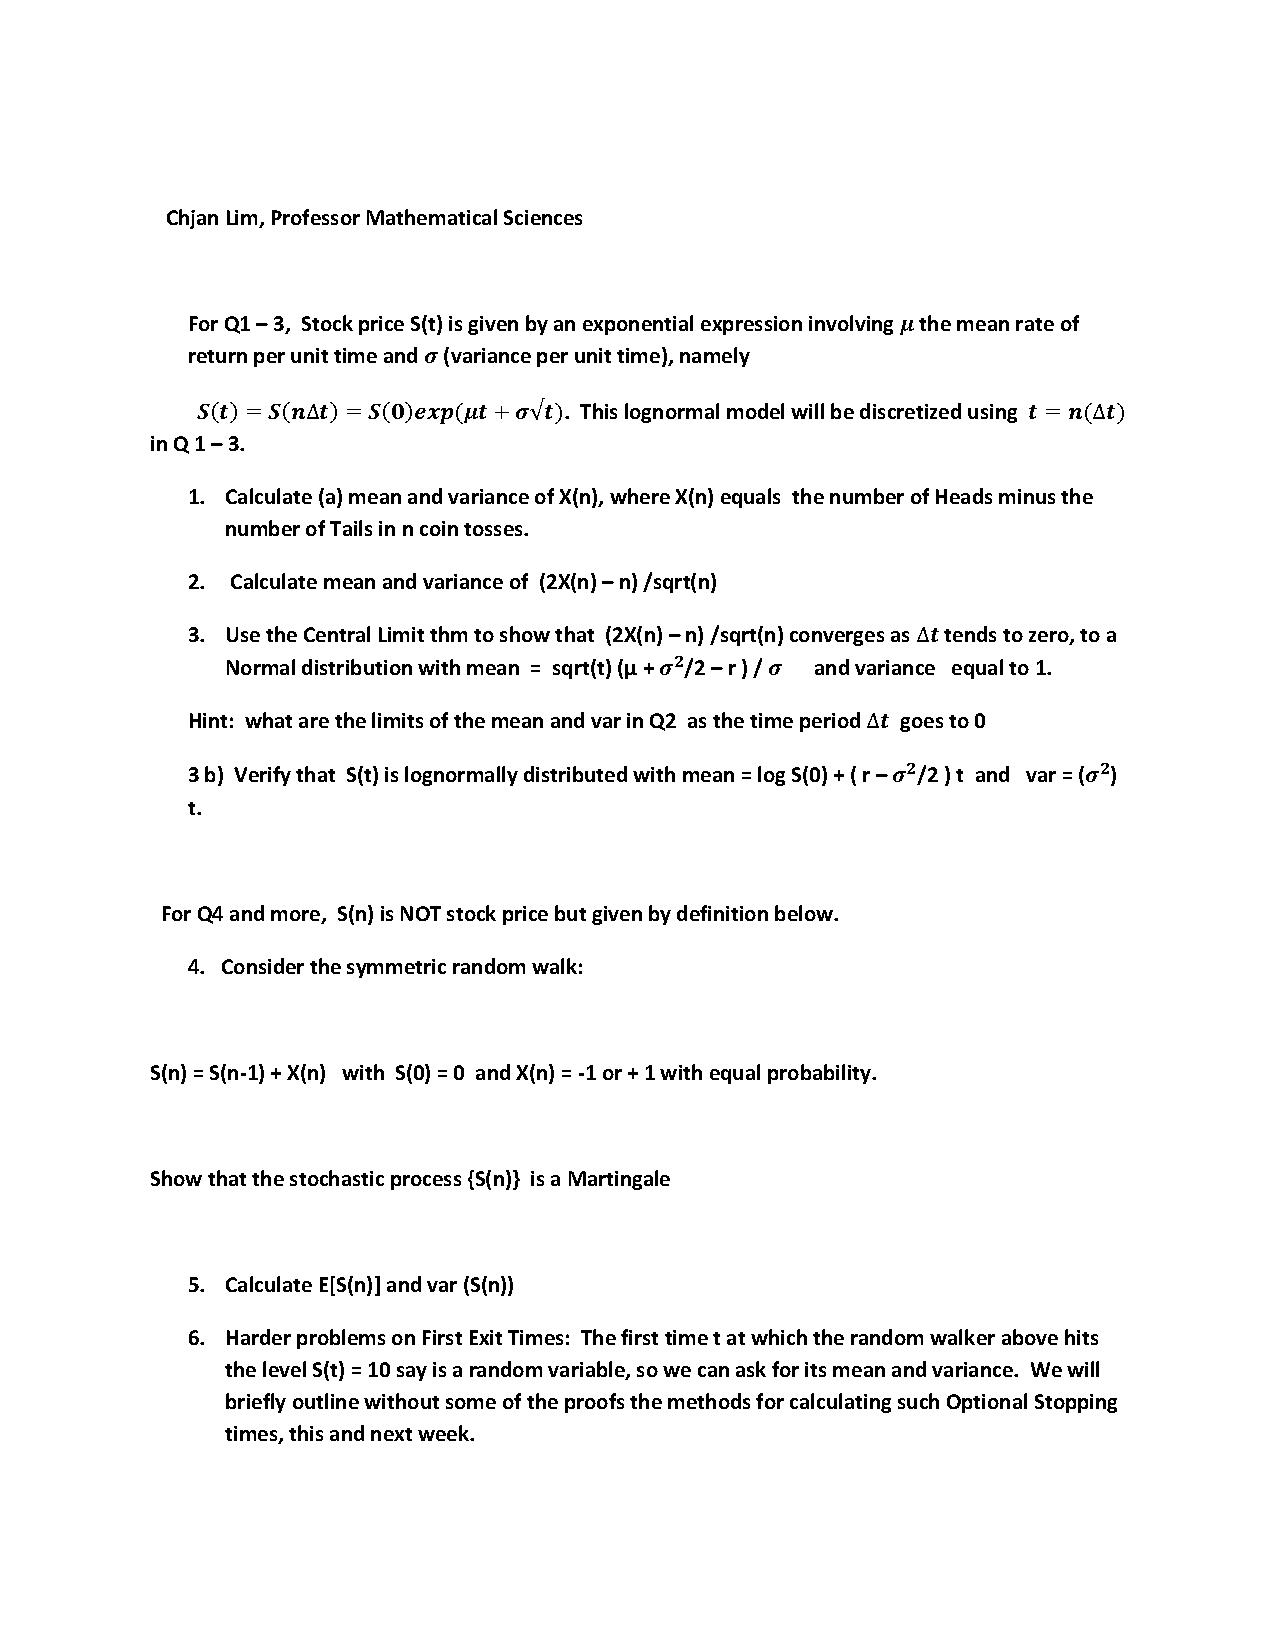
\includepdf[pages={1}]{worksheet216.pdf}
	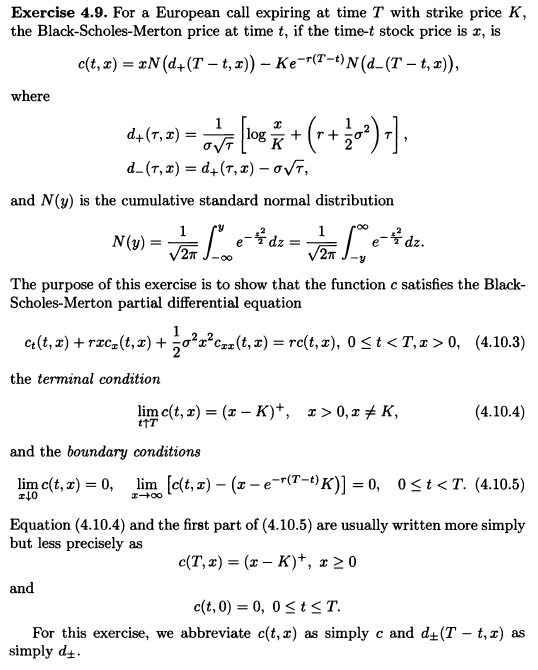
\includegraphics[width=8cm]{Ex4p9a.png}
	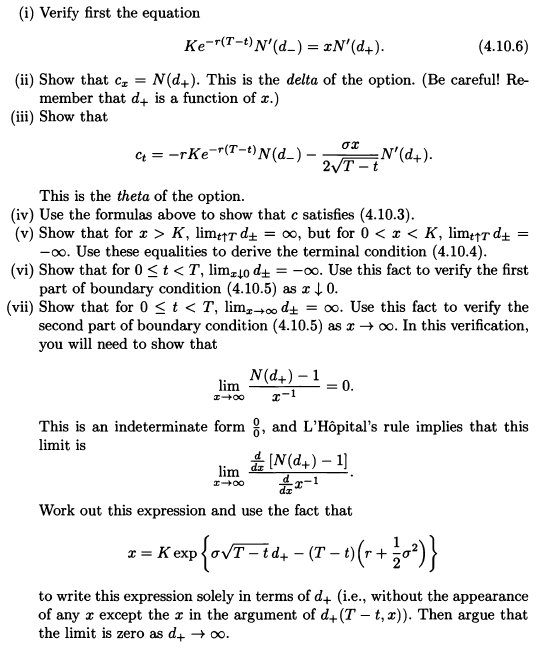
\includegraphics[width=8cm]{Ex4p9b.png}


%	\appendix
%%% \section{}
%%% \label{}
%
%%% References
%%%
%%% Following citation commands can be used in the body text:
%%% Usage of \cite is as follows:
%%%   \cite{key}         ==>>  [#]
%%%   \cite[chap. 2]{key} ==>> [#, chap. 2]
%%%
%
%%% References with bibTeX database:
%
%	\section{Reference}
	\bibliographystyle{elsarticle-harv}
	\bibliography{../MATH6740cit}
%
%%% Authors are advised to submit their bibtex database files. They are
%%% requested to list a bibtex style file in the manuscript if they do
%%% not want to use elsarticle-num.bst.
%
%%% References without bibTeX database:
%
%% \begin{thebibliography}{00}
%
%%% \bibitem must have the following form:
%%%   \bibitem{key}...
%%%
%
%% \bibitem{}
%
%% \end{thebibliography}

\end{document}



